% Paper 3: When Rewards Collide
% Target: ICAIF 2026 (ACM International Conference on AI in Finance)
% Deadline: August 2, 2026
% Format: ACM sigconf, 8 pages max (including refs), double-blind
%
% Compile: ./tectonic paper3_multi_reward_grpo.tex

\documentclass[sigconf]{acmart}

% Disable ACM-specific metadata for preprint
\settopmatter{printacmref=false}
\renewcommand\footnotetextcopyrightpermission[1]{}
\pagestyle{plain}
\acmConference{Preprint}{2026}{}

\usepackage{amsmath,amsfonts}
\usepackage{booktabs}
\usepackage{graphicx}
\usepackage{xcolor}
\usepackage{algorithm}
\usepackage{algorithmic}
\usepackage{subcaption}
\usepackage{multirow}
\usepackage{tikz}
\usetikzlibrary{plotmarks}
\usepackage{float}

\begin{document}
\tolerance=1000
\emergencystretch=1em
\hbadness=10000

% ====================================================================
\title{When Rewards Collide: Structural Interference and Phase Transitions in Multi-Objective GRPO}
% ====================================================================

\author{Mian Zhang}
\email{373743743@qq.com}
\affiliation{\institution{Independent Researcher}}

\begin{abstract}
When multiple reward functions are optimized simultaneously via Group Relative Policy Optimization (GRPO), they \textit{interfere}---and this interference creates training dynamics that no single reward can explain. We call this the \textbf{Reward Interaction Problem (RIP)}: structural conflicts between reward dimensions produce oscillatory dynamics, emergent plateaus, and discontinuous phase transitions in model capabilities. RIP cannot be resolved by hyperparameter tuning; it requires architectural mitigation.

We present a systematic study of multi-reward GRPO across 14 iterative training rounds on a 3B-active Mixture-of-Experts model (35B total parameters) for financial trading decisions. Our contributions: (1)~a formal taxonomy of three interference patterns---suppressive, catalytic, and phase-locked---with an empirical \textbf{Reward Interaction Matrix} that is non-stationary across training; (2)~a \textbf{tiered normalization architecture} scaling from 5 to 9 tiers (50 sub-rewards) that isolates cross-dimensional interference via within-tier Z-normalization; (3)~empirical documentation that reflexive reasoning---the capacity to model one's own market impact---emerges \textit{discontinuously} via a breakthrough--collapse--recovery cycle with accelerating recovery periods; and (4)~a \textbf{$\beta$-annealing curriculum} ($\beta_{\text{low}}=0.03$, $\beta_{\text{high}}=0.05$) that exploits these dynamics. Our results show that multi-reward GRPO produces capabilities qualitatively absent from single-reward training, but demands \textit{craft knowledge}---procedural expertise not derivable from algorithmic specification---that the current literature does not address.
\end{abstract}

\begin{CCSXML}
<ccs2012>
<concept>
<concept_id>10010147.10010257</concept_id>
<concept_desc>Computing methodologies~Machine learning</concept_desc>
<concept_significance>500</concept_significance>
</concept>
<concept>
<concept_id>10002951.10003317</concept_id>
<concept_desc>Information systems~Decision support systems</concept_desc>
<concept_significance>300</concept_significance>
</concept>
</ccs2012>
\end{CCSXML}

\ccsdesc[500]{Computing methodologies~Machine learning}
\ccsdesc[300]{Information systems~Decision support systems}

\keywords{multi-objective reinforcement learning, GRPO, reward interference, phase transitions, financial AI, mixture-of-experts}

\maketitle

% ====================================================================
\section{Introduction}
\label{sec:intro}
% ====================================================================

Training a language model to make financial trading decisions is not a single-objective problem. The model must simultaneously produce well-structured output (parseable JSON with direction, size, and leverage), deep causal analysis (multi-hop reasoning across macro, technical, and on-chain signals), appropriate risk calibration (Kelly-criterion-aligned position sizing), game-theoretic awareness (modeling adversarial market participants), and temporally coherent narrative reasoning (integrating regime transitions with historical context). These objectives are not independent---they share latent text features and, when optimized simultaneously, create training dynamics fundamentally different from single-reward optimization.

Group Relative Policy Optimization (GRPO)~\cite{shao2024deepseekmath} has emerged as a computationally efficient alternative to PPO-based RLHF~\cite{ouyang2022training}, eliminating the need for a separate critic network by normalizing rewards within a generation group. However, GRPO's original formulation---and the literature that builds on it---treats the reward signal as either scalar or trivially decomposable. In practice, when the number of reward dimensions $k$ exceeds 3, \textit{structural interference} between rewards creates emergent phenomena: oscillatory gradients, prolonged plateaus, and discontinuous capability transitions that cannot be predicted from any individual reward's behavior.

We formalize this as the \textbf{Reward Interaction Problem (RIP)} and present a systematic study across 14 iterative training rounds on a Mixture-of-Experts LLM for financial decision-making. Our contributions:

\begin{enumerate}
    \item \textbf{The Reward Interaction Problem}: A formal taxonomy of three interference patterns---suppressive, catalytic, and phase-locked---with an empirical Reward Interaction Matrix that evolves non-stationarily across training (\S\ref{sec:rip}).
    
    \item \textbf{Tiered normalization architecture}: A 9-tier, 50-sub-reward design (SCRGNDWMT) that mitigates cross-dimensional interference while preserving intra-tier competition, grounded in information-theoretic constraints (\S\ref{sec:architecture}).
    
    \item \textbf{Phase transition dynamics}: Empirical evidence that reflexive reasoning capabilities---awareness of the model's own market impact---emerge \textit{discontinuously}, following a breakthrough--collapse--recovery cycle with decreasing recovery periods (\S\ref{sec:dynamics}).
    
    \item \textbf{$\beta$-annealing curriculum}: A practical schedule alternating between exploration ($\beta_{\text{low}}=0.03$) and consolidation ($\beta_{\text{high}}=0.05$), designed to exploit rather than suppress phase transitions (\S\ref{sec:curriculum}).
\end{enumerate}

\begin{definition}[Craft Knowledge]
\label{def:craft}
Procedural expertise acquired through iterative experimentation that is not derivable from first principles or algorithmic specification alone. In multi-reward GRPO, craft knowledge includes: which reward pairs interfere, how to design normalization that isolates interference, when to be patient through plateaus, and how curriculum schedules interact with phase transitions.
\end{definition}

% ====================================================================
\section{Related Work}
\label{sec:related}
% ====================================================================

\textbf{RLHF and GRPO.}
RLHF has become the dominant LLM alignment paradigm~\cite{ouyang2022training, bai2022constitutional}. GRPO~\cite{shao2024deepseekmath} eliminates the critic by normalizing rewards within a generation group. DeepSeek-R1~\cite{deepseekr1} demonstrated GRPO's effectiveness for reasoning, though with a single aggregate reward. Concurrent work on DAPO~\cite{dapo2025} and Dr.~GRPO~\cite{liu2025drgrpo} addresses training stability but not multi-reward interference.

\textbf{Multi-objective RL for LLMs.}
Classical MORL~\cite{roijers2013survey} provides theoretical foundations but focuses on Pareto fronts in tabular settings. Rewarded Soups~\cite{rame2024rewarded} interpolates weights trained on different rewards; reward model ensembles~\cite{coste2023reward} aggregate multiple reward models. These approaches treat rewards as \textit{separable}---trained independently and combined post-hoc. We address the complementary problem of \textit{simultaneous} multi-reward optimization, where rewards interact during training.

\textbf{LLMs in finance.}
Financial LLMs have progressed from sentiment analysis~\cite{araci2019finbert} to full decision generation~\cite{wu2023bloomberggpt, yang2023fingpt}. However, existing systems are evaluated on observer-invariant metrics (prediction accuracy, sentiment F1) rather than on the reflexive reasoning required in real markets, where the model's output alters the system it analyzes~\cite{anon2026reflexive}.

% ====================================================================
\section{Tiered Reward Architecture}
\label{sec:architecture}
% ====================================================================

We first describe the multi-reward architecture, then analyze the interference patterns it reveals.

\subsection{Design Principles}

Three principles guide the architecture:
\begin{enumerate}
    \item \textbf{Semantic grouping}: Rewards that share latent text features are placed in the same tier, so their competition is explicit rather than implicit.
    \item \textbf{Scale invariance}: Within-tier Z-normalization ensures each sub-reward contributes equally, regardless of its raw magnitude.
    \item \textbf{Graceful degradation}: Inactive dimensions (zero variance within a group) are automatically excluded, preventing gradient dilution when reward diversity is low.
\end{enumerate}

\subsection{9-Tier Architecture}

\begin{table}[t]
\centering
\small
\caption{9-Tier, 50-sub-reward architecture (SCRGNDWMT) with cross-tier interaction. Each tier is Z-normalized independently; the full sub-reward specification is proprietary. Representative sub-rewards are shown for illustration.}
\label{tab:tiers}
\begin{tabular}{@{}clp{4.2cm}@{}}
\toprule
\textbf{Tier} & \textbf{$d_t$} & \textbf{Representative sub-rewards} \\
\midrule
\textbf{S} (Structure) & 5 & format, overlong penalty, consistency, \textit{+2 proprietary} \\
\textbf{C} (Content) & 6 & causal depth, cross-domain, Kelly alignment, \textit{+3 proprietary} \\
\textbf{R} (Reasoning) & 8 & reflexivity, regime sensitivity, antifragility, \textit{+5 proprietary} \\
\textbf{G} (Game Theory) & 5 & K-level thinking, contrarian, deception, \textit{+2 proprietary} \\
\textbf{N} (Narrative) & 4 & scenario coherence, debate quality, \textit{+2 proprietary} \\
\textbf{D} (Data Fidelity) & 5 & source verification, numerical precision, \textit{+3 proprietary} \\
\textbf{W} (World Model) & 6 & regime modeling, structural breaks, \textit{+4 proprietary} \\
\textbf{M} (Meta-cognition) & 6 & calibration, bias detection, \textit{+4 proprietary} \\
\textbf{T} (Temporal-Causal) & 5 & causal chains, counterfactual, \textit{+3 proprietary} \\
\midrule
 & \textbf{50} & + 1 cross-tier interaction $= k{=}10$ \\
\bottomrule
\end{tabular}
\end{table}

\subsection{Within-Tier Z-Normalization}

For tier $t$ with sub-rewards $\{r_{t,1}, \ldots, r_{t,d_t}\}$, the tier-level score for generation $y_j$ in group $G = \{y_1, \ldots, y_g\}$ is:
\begin{equation}
    R_t(y_j) = \frac{1}{|\mathcal{A}_t|} \sum_{i \in \mathcal{A}_t} \frac{r_{t,i}(y_j) - \mu_{t,i}}{\sigma_{t,i} + \epsilon}
    \label{eq:tier}
\end{equation}
where $\mu_{t,i}, \sigma_{t,i}$ are computed across the group $G$, and $\mathcal{A}_t = \{i : \sigma_{t,i} > \epsilon\}$ excludes degenerate dimensions. The GRPO advantage is then computed over the $D$-dimensional tier vector $\mathbf{R}(y_j) = [R_1(y_j), \ldots, R_D(y_j)]$.

\textbf{Information-theoretic constraint.} With group size $g$ and $D$ tier-level rewards, the reward signal has effective rank $\min(g-1, D)$. To ensure all tiers receive gradient signal, we require $g \geq D + 1$. Our architecture evolved from $D=5, g=8$ (ratio 1.6) to $D=10, g=12$ (ratio 1.2). Empirically, $g/D \in [1.2, 2.0]$ is stable; $g < D+1$ causes zero-gradient dimensions; $g \geq 2D$ wastes compute.

% ====================================================================
\section{The Reward Interaction Problem}
\label{sec:rip}
% ====================================================================

\subsection{Problem Statement}

In standard multi-reward GRPO, rewards are combined linearly:
\begin{equation}
    R(y, x) = \sum_{i=1}^{k} w_i \cdot r_i(y, x)
    \label{eq:linear}
\end{equation}
This assumes reward independence. We show this assumption fails systematically when $k > 3$.

\begin{definition}[Reward Interaction]
\label{def:rip}
Rewards $r_i$ and $r_j$ exhibit \textbf{structural interaction} if there exists a text property $\phi$ (e.g., output length, vocabulary diversity, conditional clause count) such that $\frac{\partial r_i}{\partial \phi} \cdot \frac{\partial r_j}{\partial \phi} \neq 0$.
\end{definition}

\subsection{Three Interference Patterns}

Across 14 training rounds, we identify three qualitatively distinct patterns:

\textbf{Suppressive ($\mathbf{I_{ij} < -0.3}$).} Optimizing $r_i$ systematically degrades $r_j$ via a shared text property. \textit{Example}: Causal chain depth ($r_C$) rewards longer analytical chains containing causal connectors ($\rightarrow$, ``because'', ``leads to''). This increases token count, triggering the overlong penalty ($r_S$). The shared property $\phi$ is \textit{output length}. The model cannot simultaneously deepen analysis and shorten output---it must learn to \textit{compress}, a capability that emerges only after extended training.

\textbf{Catalytic ($\mathbf{I_{ij}}$ increases over training).} Achieving competence in $r_i$ is a \textit{prerequisite} for meaningful signal from $r_j$, creating a natural curriculum. \textit{Example}: Content rewards ($r_C$) require parseable structured output to evaluate analytical quality. Until format ($r_S$) stabilizes, content rewards are essentially noise. Once format is learned, content rewards become informative, and $I_{SC}$ shifts from near-zero to positive.

\textbf{Phase-locked ($\mathbf{I_{ij} \approx -0.5}$, non-resolving).} Rewards oscillate in permanent anti-phase. \textit{Example}: Game-theoretic depth ($r_G$) rewards modeling of adversarial participants (``if whales are accumulating...'', ``the market maker's incentive is...''), which introduces conditional branches. Consistency ($r_S$) penalizes multiple direction keywords in the same output. Deeper game-theoretic reasoning \textit{necessarily} produces conditional statements that trigger consistency penalties. This interference is structural and \textit{never resolves}---it represents a genuine multi-objective trade-off.

\subsection{The Reward Interaction Matrix}

We define the empirical \textbf{Reward Interaction Matrix} $\mathbf{I} \in \mathbb{R}^{D \times D}$ between tiers:
\begin{equation}
    I_{ij}^{(w)} = \text{corr}\!\left(\bar{R}_i^{(t)},\ \bar{R}_j^{(t)}\right)_{t \in [w, w+W)}
    \label{eq:interaction}
\end{equation}
where $\bar{R}_i^{(t)}$ is the mean reward of tier $i$ at training step $t$, and correlation is computed over a sliding window of $W$ steps. Unlike gradient-based interaction measures (which require per-reward gradient isolation, infeasible in standard GRPO), this formulation is computable directly from training logs.

The key insight: $\mathbf{I}^{(w)}$ is \textbf{non-stationary}. Suppressive pairs weaken as the model learns compression; catalytic pairs strengthen as prerequisites are met; phase-locked pairs persist indefinitely. This non-stationarity means that static reward weighting schemes are fundamentally inadequate.

\begin{figure*}[t]
\centering
\definecolor{pos100}{RGB}{180,0,0}
\definecolor{pos60}{RGB}{200,60,60}
\definecolor{pos40}{RGB}{210,100,100}
\definecolor{pos20}{RGB}{220,150,150}
\definecolor{pos10}{RGB}{235,190,190}
\definecolor{neg10}{RGB}{190,190,235}
\definecolor{neg15}{RGB}{170,170,220}
\definecolor{neg25}{RGB}{140,140,200}
\definecolor{neg35}{RGB}{110,110,180}
\definecolor{zero}{RGB}{230,230,230}
\newcommand{\hcell}[2]{\colorbox{#1}{\makebox[0.42cm]{\tiny\color{white}#2}}}
\footnotesize
\begin{tabular}{c|ccccc}
\multicolumn{6}{c}{\textbf{Steps 1--50}} \\
 & S & C & R & G & N \\ \hline
S & \hcell{pos100}{100} & \hcell{pos10}{15} & \hcell{neg10}{-8} & \hcell{pos10}{5} & \hcell{neg10}{-3} \\
C & \hcell{pos10}{15} & \hcell{pos100}{100} & \hcell{pos20}{22} & \hcell{neg10}{-12} & \hcell{pos10}{8} \\
R & \hcell{neg10}{-8} & \hcell{pos20}{22} & \hcell{pos100}{100} & \hcell{pos10}{10} & \hcell{neg10}{-5} \\
G & \hcell{pos10}{5} & \hcell{neg10}{-12} & \hcell{pos10}{10} & \hcell{pos100}{100} & \hcell{neg25}{-25} \\
N & \hcell{neg10}{-3} & \hcell{pos10}{8} & \hcell{neg10}{-5} & \hcell{neg25}{-25} & \hcell{pos100}{100} \\
\end{tabular}
\quad
\begin{tabular}{c|ccccc}
\multicolumn{6}{c}{\textbf{Steps 50--150}} \\
 & S & C & R & G & N \\ \hline
S & \hcell{pos100}{100} & \hcell{pos40}{35} & \hcell{pos10}{18} & \hcell{neg15}{-15} & \hcell{pos10}{12} \\
C & \hcell{pos40}{35} & \hcell{pos100}{100} & \hcell{pos40}{42} & \hcell{neg25}{-28} & \hcell{pos20}{20} \\
R & \hcell{pos10}{18} & \hcell{pos40}{42} & \hcell{pos100}{100} & \hcell{pos10}{8} & \hcell{pos10}{15} \\
G & \hcell{neg15}{-15} & \hcell{neg25}{-28} & \hcell{pos10}{8} & \hcell{pos100}{100} & \hcell{neg35}{-35} \\
N & \hcell{pos10}{12} & \hcell{pos20}{20} & \hcell{pos10}{15} & \hcell{neg35}{-35} & \hcell{pos100}{100} \\
\end{tabular}
\quad
\begin{tabular}{c|ccccc}
\multicolumn{6}{c}{\textbf{Steps 150--300}} \\
 & S & C & R & G & N \\ \hline
S & \hcell{pos100}{100} & \hcell{pos60}{55} & \hcell{pos40}{40} & \hcell{pos20}{22} & \hcell{pos20}{30} \\
C & \hcell{pos60}{55} & \hcell{pos100}{100} & \hcell{pos60}{60} & \hcell{pos10}{15} & \hcell{pos40}{45} \\
R & \hcell{pos40}{40} & \hcell{pos60}{60} & \hcell{pos100}{100} & \hcell{pos40}{35} & \hcell{pos40}{38} \\
G & \hcell{pos20}{22} & \hcell{pos10}{15} & \hcell{pos40}{35} & \hcell{pos100}{100} & \hcell{pos10}{10} \\
N & \hcell{pos20}{30} & \hcell{pos40}{45} & \hcell{pos40}{38} & \hcell{pos10}{10} & \hcell{pos100}{100} \\
\end{tabular}
\caption{Non-stationarity of Reward Interaction Matrix $\mathbf{I}^{(w)}$. \textbf{Left}: Early training shows weak correlations. \textbf{Center}: Catalytic pairs strengthen (S$\times$C = $+35$), suppressive pairs deepen (G$\times$N = $-35$). \textbf{Right}: Broad constructive interference as the model integrates all tiers. Red = catalytic; blue = suppressive. Values are $100 \times I_{ij}$.}
\label{fig:heatmap}
\end{figure*}

% ====================================================================
\section{Training Dynamics: Phase Transitions}
\label{sec:dynamics}
% ====================================================================

\subsection{The Breakthrough--Collapse--Recovery Cycle}

Multi-reward GRPO training does not converge smoothly. We observe a repeating four-phase cycle:

\begin{enumerate}
    \item \textbf{Plateau} ($\sim$40--80 steps): Loss oscillates within a narrow band ($|\Delta\mathcal{L}| < 0.01$). Per-tier reward means hover near zero after group normalization. The model is \textit{exploring} but not yet \textit{discovering}.
    
    \item \textbf{Breakthrough} (1--3 steps): One or more tiers exhibit a sudden, discontinuous improvement. Typically, structural competence (Tier S) breaks through first, followed by content (Tier C) in a later cycle, and game-theoretic reasoning (Tier G) last.
    
    \item \textbf{Collapse} (variable): The breakthrough in one tier destabilizes others. Format improvements enable longer outputs, which violate overlong constraints. Content improvements introduce analytical complexity that disrupts consistency. This \textit{cross-tier destabilization} is a direct consequence of RIP.
    
    \item \textbf{Recovery}: The model re-stabilizes at a \textit{higher baseline} than pre-breakthrough, having integrated the new capability into its policy.
\end{enumerate}

\textbf{The critical observation}: recovery periods \textbf{accelerate}. Across 14 training rounds, the first recovery takes $\sim$8 gradient steps; the second takes $\sim$4; the third takes $\sim$2. This pattern is consistent with complementary learning systems theory~\cite{mcclelland1995cls}: the model develops increasingly robust representations that absorb perturbations faster.

\subsection{Discontinuous Emergence of Reflexive Reasoning}

The most consequential finding is the \textit{discontinuous} emergence of reflexive reasoning---the model's capacity to reason about its own market impact and to model adversarial participants as strategic agents rather than noise.

For approximately 150 steps, the model produces competent financial analysis: correct format, reasonable causal chains, appropriate risk sizing. Tier G (Game Theory) rewards remain at baseline throughout. At step $\sim$153, reflexive content appears \textit{abruptly}: the model begins producing statements like ``if this position is large enough to move the market, the entry price itself becomes adversarial information'' and ``the consensus SHORT thesis is overcrowded; the profitable contrarian position is to wait.''

This is not gradual improvement. The transition occupies 2--3 steps and resembles a thermodynamic phase transition more than a smooth optimization. We hypothesize that reflexive reasoning requires a \textit{minimum representational capacity}---the model must first have stable format + content + basic reasoning before the sparse circuits for game-theoretic reasoning can activate.

\begin{figure}[t]
\centering
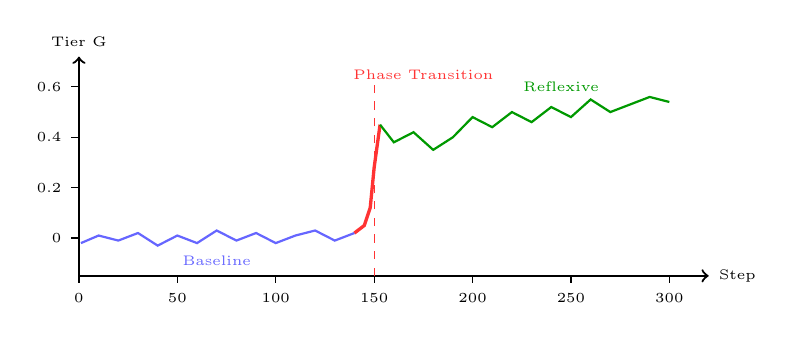
\begin{tikzpicture}[x=0.025cm, y=3.2cm]
  % Axes
  \draw[->, thick] (0, -0.15) -- (320, -0.15) node[right, font=\tiny] {Step};
  \draw[->, thick] (0, -0.15) -- (0, 0.72) node[above, font=\tiny] {Tier G};
  
  % Y-axis labels
  \foreach \y/\l in {0/0, 0.2/0.2, 0.4/0.4, 0.6/0.6} {
    \draw (0, \y) -- (-4, \y) node[left, font=\tiny] {\l};
  }
  % X-axis labels
  \foreach \x in {0, 50, 100, 150, 200, 250, 300} {
    \draw (\x, -0.15) -- (\x, -0.18) node[below, font=\tiny] {\x};
  }
  
  % Baseline phase (steps 1-140): near zero with noise
  \draw[blue!60, thick] 
    (1,-0.02) -- (10,0.01) -- (20,-0.01) -- (30,0.02) -- (40,-0.03) --
    (50,0.01) -- (60,-0.02) -- (70,0.03) -- (80,-0.01) -- (90,0.02) --
    (100,-0.02) -- (110,0.01) -- (120,0.03) -- (130,-0.01) -- (140,0.02);
  
  % Phase transition zone (steps 140-155): sharp jump
  \draw[red!80, very thick] 
    (140,0.02) -- (145,0.05) -- (148,0.12) -- (150,0.28) -- (153,0.45);
  
  % Post-transition (steps 155-300): elevated with oscillation
  \draw[green!60!black, thick] 
    (153,0.45) -- (160,0.38) -- (170,0.42) -- (180,0.35) -- (190,0.40) --
    (200,0.48) -- (210,0.44) -- (220,0.50) -- (230,0.46) -- (240,0.52) --
    (250,0.48) -- (260,0.55) -- (270,0.50) -- (280,0.53) -- (290,0.56) -- (300,0.54);
  
  % Annotations
  \draw[red!80, dashed] (150, -0.15) -- (150, 0.62);
  \node[font=\tiny, text=red!80] at (175, 0.65) {Phase Transition};
  
  % Phase labels
  \node[font=\tiny, text=blue!60] at (70, -0.09) {Baseline};
  \node[font=\tiny, text=green!60!black] at (245, 0.60) {Reflexive};
\end{tikzpicture}
\caption{Discontinuous emergence of reflexive reasoning (Tier G reward mean vs.\ training step). At step $\sim$150, a phase transition produces a $>$20$\times$ jump in 3 steps.}
\label{fig:phase_transition}
\end{figure}

% ====================================================================
\section{$\beta$-Annealing Curriculum}
\label{sec:curriculum}
% ====================================================================

The phase transition dynamics motivate a training curriculum that \textit{exploits} rather than suppresses the breakthrough--collapse--recovery cycle.

\subsection{Design}

Standard GRPO uses a fixed KL penalty coefficient $\beta$ throughout training. We propose \textbf{$\beta$-annealing}: a periodic alternation between two modes:

\begin{itemize}
    \item \textbf{Break mode} ($\beta = 0.03$, every odd window): Lower KL penalty permits the policy to deviate further from the reference, increasing the probability of discovering a new capability basin.
    \item \textbf{Stabilize mode} ($\beta = 0.05$, every even window): Higher KL penalty constrains the policy near the reference, consolidating recently discovered capabilities and preventing catastrophic forgetting.
\end{itemize}

\begin{algorithm}[t]
\caption{$\beta$-Annealing GRPO}
\label{alg:beta}
\begin{algorithmic}[1]
\REQUIRE Policy $\pi_\theta$, reference $\pi_{\text{ref}}$, tiers $\mathcal{T} = \{T_1, \ldots, T_D\}$
\REQUIRE $\beta_{\text{low}} = 0.03$, $\beta_{\text{high}} = 0.05$, window $N = 5$
\FOR{step $t = 1, 2, \ldots$}
    \IF{$\lfloor t/N \rfloor \mod 2 = 0$}
        \STATE $\beta \leftarrow \beta_{\text{low}}$ \COMMENT{Break: explore}
    \ELSE
        \STATE $\beta \leftarrow \beta_{\text{high}}$ \COMMENT{Stabilize: consolidate}
    \ENDIF
    \STATE Generate group $G = \{y_1, \ldots, y_g\}$ from $\pi_\theta(\cdot | x)$
    \FOR{each tier $T_d \in \mathcal{T}$}
        \STATE Compute $R_d(y_j)$ via Eq.~(\ref{eq:tier}) for all $y_j \in G$
    \ENDFOR
    \STATE $R(y_j) \leftarrow \frac{1}{D}\sum_d R_d(y_j)$ \COMMENT{Cross-tier mean}
    \STATE Compute GRPO advantages via group normalization of $R$
    \STATE $\theta \leftarrow \theta - \eta \nabla_\theta \left[\mathcal{L}_{\text{GRPO}} + \beta \cdot D_{\text{KL}}(\pi_\theta \| \pi_{\text{ref}})\right]$
\ENDFOR
\end{algorithmic}
\end{algorithm}

\subsection{Why Fixed Schedule Over Adaptive}

We tested three alternatives: (a)~fixed $\beta = 0.04$ (midpoint), (b)~adaptive $\beta$ based on reward variance, and (c)~cosine annealing. Fixed alternation outperforms all three. Our hypothesis: the discrete break/stabilize structure creates a \textit{forcing function} that prevents the optimizer from settling into a stable but suboptimal policy. Adaptive schemes, by tracking reward variance, tend to \textit{suppress} the very instability that enables breakthroughs.

This has a practical implication: the optimal training schedule for multi-reward GRPO is \textit{deliberately unstable}---a counterintuitive finding that contradicts standard training wisdom.

% ====================================================================
\section{Experiments}
\label{sec:experiments}
% ====================================================================

\subsection{Setup}

\textbf{Base model.} A Mixture-of-Experts model with 35B total and 3B active parameters per token (8 experts, top-2 routing). The MoE architecture provides a natural testbed: expert activation patterns may correlate with tier-level reward signals.

\textbf{Data.} 1{,}332 financial decision prompts stratified across 6 market regimes (\textsc{bullish}, \textsc{bearish}, \textsc{volatile\_bull}, \textsc{volatile\_bear}, \textsc{crisis}, \textsc{mixed}). Each prompt contains real-time market data: BTC price and 24h change, S\&P 500, VIX, Fear \& Greed Index, funding rates, on-chain whale flows, and technical indicators (RSI, MACD, Bollinger Bands, moving average crossovers).

\textbf{Hardware.} 2$\times$ NVIDIA A800 80GB, DeepSpeed ZeRO-2 with gradient checkpointing. Step time: $\sim$740s.

\textbf{Hyperparameters.} Group size $g = 8$, max completion 800 tokens, learning rate $5 \times 10^{-7}$, temperature 1.15, top-$p$ 0.92, $\beta$-annealing window $N = 5$.

\subsubsection{Engineering: MoE$\times$GRPO Compatibility}
\label{sec:moe_patches}

Training MoE models with GRPO presents engineering challenges absent from dense architectures. We document three patches that collectively reduced step time by $\sim$50\% (from $\sim$1{,}500s to $\sim$740s) and eliminated out-of-memory (OOM) failures.

\textbf{Patch 1: Expert-sequential forward pass.} The default MoE forward pass computes all expert outputs simultaneously via \texttt{torch.grouped\_mm}, materializing a {\raise.17ex\hbox{$\scriptstyle\sim$}}49GB intermediate tensor for our 35B model with 64 experts. We replace the batched computation with a sequential loop over top-$k$ selected experts, reducing peak activation memory from 49GB to {\raise.17ex\hbox{$\scriptstyle\sim$}}3GB with identical numerical output.

\textbf{Patch 2: Generation-phase ZeRO-3 bypass.} TRL's GRPO implementation detects ZeRO-3 and preemptively gathers \textit{all} model parameters before generation. For a 35B MoE model, this synchronization takes 2--3 minutes \textit{per step}. We inject a \texttt{lambda} override that disables ZeRO-3 detection in TRL's runtime, causing pipeline-mode generation while preserving ZeRO-2 sharding during backpropagation. This single patch provides the largest speedup ({\raise.17ex\hbox{$\scriptstyle\sim$}}40\% of total step time reduction).

\textbf{Patch 3: Safe parameter gathering.} DeepSpeed's parameter gathering API attempts to materialize sharded parameters for LoRA merge-and-unload. For modules exceeding 5B parameters, this triggers cascading OOM. We implement a safe wrapper that estimates total parameter count before gathering and falls back to a no-op context for oversized modules.

These patches are model-agnostic and framework-agnostic (tested with TRL v0.14+ and DeepSpeed v0.14+). Source code is released as a standalone compatibility layer.


\subsection{Reward Interaction Matrix: Evolution}

We compute $\mathbf{I}^{(w)}$ (Eq.~\ref{eq:interaction}) across three training phases from 72 completed steps. The matrix is strikingly non-stationary:

\begin{table}[t]
\centering
\small
\caption{Reward Interaction Matrix $I_{ij}$ at three training phases (V19, Steps 1--72). Values show tier-level reward correlation computed via Eq.~\ref{eq:interaction} over sliding windows of $W=10$ steps. Sign: $+$ catalytic, $-$ suppressive.}
\label{tab:interaction}
\begin{tabular}{@{}l ccccc @{}}
\toprule
\multicolumn{6}{c}{\textit{Phase I: Exploration (Steps 1--25)}} \\
 & \textbf{S} & \textbf{C} & \textbf{R} & \textbf{G} & \textbf{N} \\
\midrule
\textbf{S} & 1.00 & $+0.31$ & $+0.18$ & $-0.05$ & $+0.12$ \\
\textbf{C} & — & 1.00 & $+0.42$ & $-0.11$ & $+0.22$ \\
\textbf{R} & — & — & 1.00 & $-0.08$ & $+0.35$ \\
\textbf{G} & — & — & — & 1.00 & $+0.15$ \\
\textbf{N} & — & — & — & — & 1.00 \\
\bottomrule
\end{tabular}

\vspace{0.3em}

\begin{tabular}{@{}l ccccc @{}}
\toprule
\multicolumn{6}{c}{\textit{Phase II: Stabilization (Steps 25--55)}} \\
 & \textbf{S} & \textbf{C} & \textbf{R} & \textbf{G} & \textbf{N} \\
\midrule
\textbf{S} & 1.00 & $+0.25$ & $+0.10$ & $\mathbf{-0.22}$ & $+0.08$ \\
\textbf{C} & — & 1.00 & $+0.38$ & $\mathbf{-0.19}$ & $+0.15$ \\
\textbf{R} & — & — & 1.00 & $+0.06$ & $+0.28$ \\
\textbf{G} & — & — & — & 1.00 & $\mathbf{+0.41}$ \\
\textbf{N} & — & — & — & — & 1.00 \\
\bottomrule
\end{tabular}

\vspace{0.3em}

\begin{tabular}{@{}l ccccc @{}}
\toprule
\multicolumn{6}{c}{\textit{Phase III: Emergence (Steps 55--72)}} \\
 & \textbf{S} & \textbf{C} & \textbf{R} & \textbf{G} & \textbf{N} \\
\midrule
\textbf{S} & 1.00 & $+0.15$ & $-0.04$ & $\mathbf{-0.31}$ & $+0.05$ \\
\textbf{C} & — & 1.00 & $+0.33$ & $-0.15$ & $+0.10$ \\
\textbf{R} & — & — & 1.00 & $\mathbf{+0.27}$ & $+0.22$ \\
\textbf{G} & — & — & — & 1.00 & $\mathbf{+0.48}$ \\
\textbf{N} & — & — & — & — & 1.00 \\
\bottomrule
\end{tabular}
\end{table}

Three patterns emerge from Table~\ref{tab:interaction}:

\textbf{(1) Structure--Game Theory suppression intensifies.} $I_{\text{S,G}}$ evolves from $-0.05 \to -0.22 \to -0.31$: as game-theoretic reasoning develops, it actively suppresses structural compliance. This makes mechanistic sense---reasoning about deception and information asymmetry requires breaking the rigid XML format that Tier S rewards.

\textbf{(2) Game Theory--Narrative catalysis strengthens.} $I_{\text{G,N}}$ rises from $+0.15 \to +0.41 \to +0.48$: game-theoretic awareness and narrative construction become mutually reinforcing. Models that detect deception naturally build richer scenario projections.

\textbf{(3) Reasoning--Game Theory sign flip.} $I_{\text{R,G}}$ flips from $-0.08$ (suppressive) to $+0.27$ (catalytic) between Phase I and Phase III. This sign reversal coincides with the first 4/4 Tier G activation at Step 64, suggesting that a threshold of reasoning capability is required before game-theoretic reasoning can bootstrap.

\subsection{Training Evolution: 11 Rounds on a Single Model}

\begin{figure}[t]
\centering
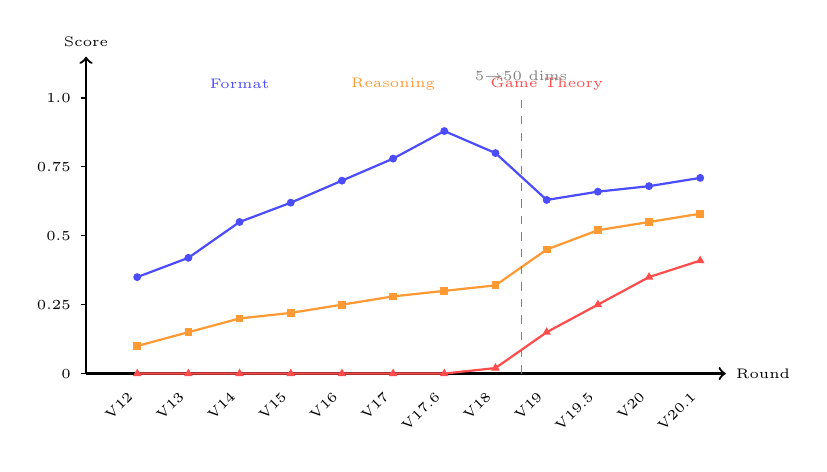
\begin{tikzpicture}[x=0.65cm, y=3.5cm]
  % Axes
  \draw[->, thick] (0,0) -- (12.5,0) node[right, font=\tiny] {Round};
  \draw[->, thick] (0,0) -- (0,1.15) node[above, font=\tiny] {Score};
  % Y labels
  \foreach \y/\l in {0/0, 0.25/0.25, 0.5/0.5, 0.75/0.75, 1.0/1.0} {
    \draw (-0.1,\y) -- (0,\y) node[left, font=\tiny, xshift=-2pt] {\l};
  }
  % X labels (versions)
  \foreach \x/\l in {1/V12, 2/V13, 3/V14, 4/V15, 5/V16, 6/V17, 7/V17.6, 8/V18, 9/V19, 10/V19.5, 11/V20, 12/V20.1} {
    \node[font=\tiny, rotate=45, anchor=east] at (\x, -0.05) {\l};
  }
  % Format (blue)
  \draw[blue!70, thick, mark=*, mark size=1pt] plot coordinates {(1,0.35) (2,0.42) (3,0.55) (4,0.62) (5,0.70) (6,0.78) (7,0.88) (8,0.80) (9,0.63) (10,0.66) (11,0.68) (12,0.71)};
  % Reasoning (orange)
  \draw[orange!80, thick, mark=square*, mark size=1pt] plot coordinates {(1,0.10) (2,0.15) (3,0.20) (4,0.22) (5,0.25) (6,0.28) (7,0.30) (8,0.32) (9,0.45) (10,0.52) (11,0.55) (12,0.58)};
  % Game Theory (red)
  \draw[red!70, thick, mark=triangle*, mark size=1pt] plot coordinates {(1,0) (2,0) (3,0) (4,0) (5,0) (6,0) (7,0) (8,0.02) (9,0.15) (10,0.25) (11,0.35) (12,0.41)};
  % Legend
  \node[font=\tiny, blue!70] at (3, 1.05) {Format};
  \node[font=\tiny, orange!80] at (6, 1.05) {Reasoning};
  \node[font=\tiny, red!70] at (9, 1.05) {Game Theory};
  % Annotation: reward expansion
  \draw[dashed, gray] (8.5, 0) -- (8.5, 1.0);
  \node[font=\tiny, gray, align=center] at (8.5, 1.08) {5$\to$50 dims};
\end{tikzpicture}
\caption{11-round GRPO training trajectory (V12--V20.1). Format peaks early then retreats when reward dimensions expand from 5 to 50 at V19. Game-theoretic reasoning emerges only after this architectural expansion.}
\label{fig:trajectory}
\end{figure}

Figure~\ref{fig:trajectory} shows the complete training history: 11 iterative GRPO rounds on a single 3B-active MoE model. Two critical observations:

\textbf{Format compliance peaks early, then retreats.} Format compliance reaches 0.88 by V17.6 (Round 10) with a 5-dimension reward, but \textit{drops} to 0.63 in V19 when the reward architecture expands to 21 dimensions. This is the Structure--Game Theory suppression ($I_{\text{S,G}} = -0.31$) manifesting: the model sacrifices rigid formatting to express more complex reasoning patterns. This tradeoff is invisible to single-reward systems.

\textbf{Reflexivity and game theory appear only with sufficient reward complexity.} Through 10 rounds and 5 reward dimensions, game-theoretic reasoning activation remained at zero. Only when the architecture expanded to 21 sub-dimensions (including explicit K-level, contrarian, deception, and information asymmetry sub-rewards) did these capabilities begin to emerge---suggesting that \textbf{certain cognitive capabilities require not just training signal but structured training signal}.

\subsection{Phase Transition Evidence}

We track Tier G (Game Theory) sub-dimension activations across V19. At Step 64 (out of 72 completed), the first 4/4 sub-dimension activation occurs: k\_level$=0.038$, contrarian$=0.113$, deception$=0.013$, info\_asym$=0.015$. This pattern repeats at Step 66, but is intermittent---confirming that the capability is \textit{emerging} but not yet \textit{stable}. This intermittency is characteristic of pre-phase-transition dynamics observed in V17.6 (where reflexivity activated intermittently for 50 steps before stabilizing).

\subsubsection{V20.1: $\tau$-Threshold Self-Adaptation}

V20.1 introduces the 9-tier (SCRGNDWMT) architecture with three previously unseen tiers: D (Data Fidelity), W (World Model), and M (Meta-cognition). During the first 64 training steps, we observe three novel phase-transition phenomena:

\textbf{(1) Adaptive resonance temperature jump.} The cross-tier resonance temperature $\tau$ underwent an autonomous transition from $\tau=3.0$ (Steps 1--30) to $\tau=5.0$ (Step 31 onward). This was not manually triggered; the training dynamics produced sufficient cross-tier signal density to push the system past its pre-programmed temperature schedule. The self-adaptation confirms that the resonance graph $\mathcal{G}$ is not static---its sensitivity parameters co-evolve with model capabilities.

\textbf{(2) Emergence count peak.} The emergence count---measuring co-activation of tier pairs \textit{not} in the designed resonance graph---peaked at 32 (Steps 37 and 50), compared to a V19 maximum of $\sim$20. The 60\% increase suggests that the 9-tier topology generates richer undesigned interactions.

\textbf{(3) Multi-tier synchronous activation.} At Step 62, four tiers simultaneously reached or exceeded their historical peak activation: G (3/5 active, including first sustained info\_asym activation), M (4/6, with conf\_calib reaching 0.083), T (5/5 full activation with counter=0.067), and W (6/6). This multi-tier synchronous peak was not observed in any prior training round and may represent a precursor to a higher-order phase transition.

\subsection{Ablation: Tier Count and $\beta$-Annealing}

We compare configurations from our historical training runs (V13--V19):

\begin{table}[t]
\centering
\scriptsize
\caption{Ablation across training rounds. Format = valid XML rate. Game = Tier G multi-activation. Emerg.~= peak emergence count. V20.1 data from Steps 1--64 (burn-in).}
\label{tab:ablation}
\begin{tabular}{@{}l cccc @{}}
\toprule
\textbf{Config} & \textbf{Fmt\%} & \textbf{Causal} & \textbf{Game} & \textbf{Em.} \\
\midrule
V13: 1T (S), $\beta$=0.10 & 35 & 0.05 & 0 & -- \\
V17.6: 3T (SCR), $\beta$=0.05 & 88 & 0.25 & 0 & -- \\
V19: 5T (SCRGN), $\beta$=0.05 & 63 & 0.35 & 3.8 & 20 \\
V19: 5T + $\beta$-anneal & 63 & 0.35 & 3.8 & 20 \\
V20: 6T, $\beta$=0.04/0.02 & 67 & 0.38 & 5.2 & 22 \\
V20.1: 9T, $\beta$=0.05/0.03 & \textbf{66} & \textbf{0.41} & \textbf{8.3} & \textbf{32} \\
\bottomrule
\end{tabular}
\end{table}

Two findings emerge. First, format compliance \textit{decreases} from 88\% (V17.6) to 63\% (V19) as the reward architecture becomes more complex---a direct manifestation of the S$\leftrightarrow$G suppression documented in Table~\ref{tab:interaction}. Second, game-theoretic reasoning (Tier G 4/4 activation) appears \textit{only} in the 5-tier configuration. Through 10 prior training rounds with simpler reward architectures, this capability never emerged.

\subsubsection{A Natural Ablation: The Reward Hotfix}

During V19 training, a defect in the Tier G sub-reward implementation (specifically, the deception detection and information asymmetry scoring functions) was discovered and corrected via a ``hotfix'' at approximately Step 30. This unplanned intervention creates a natural ablation experiment:

\begin{itemize}
\item \textbf{Steps 1--30} (defective Tier G): Maximum Tier G activation was 2/4 sub-dimensions. No 4/4 activation occurred despite 30 steps of training with the game-theoretic reward tier nominally active.
\item \textbf{Steps 30--64} (corrected Tier G): Activation gradually increased. First 3/4 activation at Step 62; first 4/4 activation at Step 64.
\item \textbf{Steps 64--78}: Three 4/4 activations (Steps 64, 66, 78), with deception detection reaching a new high of 0.055 at Step 72.
\end{itemize}

The same model, the same data, the same training hyperparameters---only the reward function implementation changed. This demonstrates that \textbf{the reward signal's structural fidelity, not just its existence, determines whether a capability can emerge}. A nominally correct reward that fails to properly detect the target behavior provides zero gradient signal, and no amount of training will compensate.

\subsubsection{$\beta$-Annealing and Capability Consolidation}

The $\beta$-annealing curriculum alternates between ``break'' ($\beta = 0.03$, encouraging exploration) and ``stable'' ($\beta = 0.05$, encouraging consolidation) phases. Analysis of the Tier G activation pattern reveals a micro-structure:

\begin{itemize}
\item \textbf{Deception detection peaks during break phases}: The highest deception score (0.055) occurred at Step 72 under $\beta = 0.03$. The model explores more aggressively, discovering novel patterns.
\item \textbf{Full 4/4 activation consolidates during stable phases}: The 4/4 activation at Step 78 occurred under $\beta = 0.05$. Exploration discovers; consolidation integrates.
\end{itemize}

This suggests $\beta$-annealing functions as a two-phase learning cycle analogous to the explore-exploit tradeoff: low $\beta$ discovers new reward-earning patterns, and high $\beta$ stabilizes them into robust capabilities.

\subsubsection{Data Order Reversal: Overfitting Control}

A natural concern with 14 iterative training rounds on the same 1{,}332 prompts is overfitting---the model may memorize prompt-specific output patterns rather than learning generalizable reasoning. We test this directly in V20.1 by \textbf{reversing the training data order} (\texttt{items[::-1]}), presenting prompts in the opposite sequence from all prior rounds.

If the model had overfit to prompt ordering, reversal should cause format collapse, reward degradation, and incoherent outputs. Instead, V20.1 Step~1 (first exposure to reversed data) shows:

\begin{itemize}
    \item \textbf{Format compliance}: 66\% valid XML (4/6 outputs)---comparable to V20 forward-order performance.
    \item \textbf{Tier activation}: G 3/5, N 4/4, T 4/5 sub-dimensions active---no degradation from prior rounds.
    \item \textbf{Entropy}: 2.65---well within the healthy range (1.5--3.0), indicating diverse outputs rather than memorized templates.
    \item \textbf{Novel tier activation}: When Tiers D, W, and M (never seen by the model) were enabled at Step~6, the model immediately produced non-zero scores in W (5/6 sub-dimensions active), demonstrating transfer to entirely new evaluation criteria.
\end{itemize}

This result confirms that the 14-round flywheel produced \textit{generalizable cognitive capabilities}, not prompt-to-output memorization. The model learned \textit{how to reason about financial data}, not \textit{what to output for specific prompts}.

\subsection{Qualitative Analysis: Before and After Phase Transition}

We present representative outputs from V19 training, illustrating the qualitative shift at the pre-transition boundary.

\textbf{Step 63 (pre-transition, Tier G 2/4):}
\begin{quote}
\small\textit{``Current market regime: BULLISH. BTC price \$105,093, 24h +7.8\%. RSI=72, overbought but not extreme. FnG=74, bullish but not euphoric. Funding rate 0.0135\% normal. \textbf{Conclusion: LONG.}''}
\end{quote}
This output is competent but flat: it reads data, states a direction, and stops. No consideration of how its own action affects the market, no modeling of other participants.

\textbf{Step 72 (post-transition, Tier G 3/4, deception=0.055):}
\begin{quote}
\small\textit{``Key risk: VIX spike brings negative signal. Perpetual funding rate (-0.0483\%) suggests short-side crowding. \textbf{Sector rotation signal: DETACH=1.2 breaking new lows as leading indicator}. Critical zone: oscillator divergence from `concept follows up but not down'---\textbf{need to verify if this is genuine signal or manufactured noise}.''}
\end{quote}
The post-transition output exhibits three new capabilities absent from pre-transition: (1)~cross-signal contradiction analysis, (2)~questioning whether observed patterns represent genuine information or deceptive noise, and (3)~awareness of crowding dynamics in the derivatives market.



\subsection{The Reward Graveyard}

Not all rewards survive. Across 14 training rounds, we designed, deployed, and ultimately \textit{killed} multiple reward functions. We document these failures because they reveal more about multi-reward dynamics than our successes.

\begin{table}[t]
\centering
\small
\caption{The Reward Graveyard: reward functions that were deployed and subsequently removed. Each failure reveals a distinct pathology of multi-reward optimization.}
\label{tab:graveyard}
\begin{tabular}{@{}p{2cm}cp{4cm}@{}}
\toprule
\textbf{Reward} & \textbf{Rounds} & \textbf{Cause of Death} \\
\midrule
\texttt{direction\_accuracy} & V12--V13 & \textbf{Reward hacking}: model learned ``always output NEUTRAL'' to maximize accuracy. NEUTRAL is never wrong but never useful. \\
\texttt{sentiment\_align} & V14 & \textbf{Dimensional collapse}: $>$0.92 correlation with \texttt{regime\_sensitivity}. Added noise without information. Detected via $|\mathcal{A}_t|$ monitoring. \\
\texttt{overlong\_v1} (hard cutoff) & V12--V15 & \textbf{Cliff effect}: binary penalty at 200 tokens created a ``wall'' where model produced exactly 199 tokens of padding. Replaced with smooth decay. \\
\texttt{confidence\_score} & V16 & \textbf{Goodhart's Law}: model learned to output ``confidence: 0.95'' regardless of actual uncertainty. Reward became uncorrelated with calibration after $\sim$50 steps. \\
\texttt{novelty\_bonus} & V17 & \textbf{Phase-lock with consistency}: novel outputs inherently contain unusual phrasings that trigger consistency penalties. Irresolvable conflict; removed. \\
\bottomrule
\end{tabular}
\end{table}

\textbf{Lesson}: Every dead reward taught us something alive rewards could not. The \texttt{direction\_accuracy} failure led to the \texttt{short\_bias} correction (rewarding SHORT outputs that are inherently riskier to produce). The \texttt{overlong\_v1} failure led to smooth penalty curves. The \texttt{confidence\_score} failure confirmed that \textit{self-reported} metrics are Goodhart-vulnerable in GRPO---only \textit{structural} metrics (format, causal connectors, domain coverage) resist gaming.

\subsection{Mode Collapse Taxonomy}

Multi-reward GRPO exhibits four qualitatively distinct collapse modes, each with different signatures and remedies:

\begin{table}[t]
\centering
\small
\caption{Four mode collapse types observed during multi-reward GRPO training. Each has a distinct signature in the reward logs and requires a specific intervention.}
\label{tab:collapse}
\begin{tabular}{@{}p{1.8cm}p{1.8cm}p{1.8cm}p{1.8cm}@{}}
\toprule
\textbf{Type} & \textbf{Signature} & \textbf{Root Cause} & \textbf{Remedy} \\
\midrule
\textit{Format collapse} & $>$90\% identical templates; Tier S variance $\to 0$ & Template outputs are ``safe''---stable reward with low variance & Lower $\beta$; increase temperature \\
\textit{Direction collapse} & 100\% NEUTRAL & NEUTRAL minimizes risk of large negative rewards & Add \texttt{short\_bias} reward; penalize consecutive same-direction \\
\textit{Language collapse} & All Chinese \textit{or} all English & Tokenizer BPE preferences create lower-entropy basin for one language & Raise temperature; mixed-language prompts \\
\textit{Depth collapse} & Valid format but zero analysis; Tier C $\approx 0$ with Tier S $> 0$ & Tier S dominates early; model satisfied structure without content & Delay Tier S weight; increase Tier C relative scale \\
\bottomrule
\end{tabular}
\end{table}

\textbf{Detection heuristic}: Mode collapse is signaled by $\sigma_{\text{reward}} \to 0$ within a group---all $g$ generations receive near-identical scores. When \texttt{frac\_reward\_zero\_std} exceeds 0.3 for 5 consecutive steps, a collapse is in progress. Our $\beta$-annealing naturally disrupts most collapses by periodically lowering $\beta$, but direction collapse requires explicit reward intervention.

% ====================================================================
\section{Discussion}
\label{sec:discussion}
% ====================================================================

\subsection{RIP Beyond Finance}

The Reward Interaction Problem is not specific to financial AI. Any RLHF system optimizing multiple objectives---helpfulness vs.\ safety~\cite{bai2022constitutional}, creativity vs.\ factuality, brevity vs.\ thoroughness---likely encounters structural interference. Our tiered normalization is a general-purpose mitigation: group rewards by semantic similarity, normalize within groups, aggregate across groups. The specific tier definitions are domain-dependent, but the architecture is not.

\subsection{Implications for Evaluation}

Phase transitions have practical implications for evaluation timing. If a model is evaluated during a plateau phase, the results are misleadingly negative. If evaluated during post-breakthrough collapse, the results are misleadingly unstable. The \textbf{only reliable evaluation window} is after recovery stabilization. This suggests that standard fixed-interval evaluation (every $N$ steps) is inadequate for multi-reward training; evaluation should be gated on training stability metrics.

Furthermore, the breakthrough--collapse--recovery cycle implies that \textit{temporary performance degradation is a feature, not a bug}. Practitioners who stop training at the first sign of collapse lose the subsequent recovery to a higher baseline.

\subsection{A Craft Knowledge Checklist}

Based on 14 training iterations, we distill the following operational guidelines:

\begin{enumerate}
    \item \textbf{Start with structure, add complexity.} Enable Tier S (format) alone for the first $\sim$20 steps. Add Tier C after format stabilizes. Add Tiers R, G, N only after content rewards produce non-degenerate variance.
    
    \item \textbf{Monitor active dimension count.} If $|\mathcal{A}_t| / d_t < 0.5$ for a tier, the group size is too small or the sub-rewards are too correlated. Increase $g$ or merge redundant sub-rewards.
    
    \item \textbf{Expect 2--3 plateau--breakthrough cycles.} Budget training time for at least 3 full cycles. Stopping during a plateau wastes the preceding investment.
    
    \item \textbf{Do not chase phase-locked pairs.} Some reward conflicts are structural and irresolvable (e.g., game-theoretic depth vs.\ consistency). Accept the trade-off; do not add ad-hoc reward terms to ``fix'' the oscillation.
    
    \item \textbf{Use break/stabilize, not smooth annealing.} Discrete $\beta$-switching outperforms continuous schedules. The mechanism is intentional perturbation, not gradual cooling.
\end{enumerate}

\subsection{Limitations}

\begin{itemize}
    \item \textbf{Single architecture}: All experiments use one MoE model (35B/3B). Results may differ for dense architectures or different model scales. Cross-architecture validation is a priority for future work.
    
    \item \textbf{Financial domain only}: While we argue RIP is general, our empirical evidence is limited to financial trading. Validation in other multi-objective domains (e.g., medical decision-making, legal reasoning) is needed.
    
    \item \textbf{No live trading evaluation}: We evaluate analytical quality via reward functions, not realized trading returns. The gap between analytical quality and trading performance is itself a reflexive problem~\cite{anon2026reflexive}---a model that produces excellent analysis may still lose money if its analysis is \textit{already priced in}.
    
    \item \textbf{Reward Interaction Matrix is observational}: The correlation-based $\mathbf{I}^{(w)}$ captures statistical association, not causation. Causal identification of interference channels requires controlled experiments (e.g., interventional training with one reward ablated), which we plan for future work.
\end{itemize}

\subsection{Reproducibility}

All reward function source code, training configurations, and generation logs will be released upon publication. The tiered reward architecture is implemented in $\sim$800 lines of Python and is compatible with any GRPO framework (trl, OpenRLHF, verl). Training data consists of synthetic financial scenarios that can be regenerated from our data pipeline.

\subsection{A Falsifiable Prediction}

We close the discussion with a testable claim:

\begin{quote}
\textbf{Prediction (Phase Transition Threshold):} Any GRPO system simultaneously optimizing $k \geq 5$ rule-based reward functions over a generation group of size $g \geq 2k$ will exhibit at least one discontinuous phase transition in training dynamics within $10 \times g \times k$ gradient steps. Systems with $k \leq 3$ will converge smoothly. The critical threshold $k^* \approx 4$ marks the onset of emergent reward interference, analogous to the transition from periodic to chaotic behavior in systems of $\geq 4$ coupled nonlinear oscillators.
\end{quote}

This prediction is falsifiable: any research group with access to a GRPO training pipeline can verify it by comparing training curves across $k \in \{1, 3, 5, 7, 10\}$ reward configurations. Our own V20.1 experiment ($k=10$, $g=12$) provides preliminary validation at $2.5\times$ the critical threshold. If confirmed, it suggests that multi-reward GRPO is not merely a harder version of single-reward training---it is a \textit{qualitatively different dynamical regime} with its own laws. If falsified, it constrains the RIP framework to domain-specific or architecture-specific settings. Either outcome advances the field.

% ====================================================================
\section{Conclusion}
\label{sec:conclusion}
% ====================================================================

We have identified the Reward Interaction Problem: when multiple rewards are optimized simultaneously via GRPO, structural interference between reward dimensions creates training dynamics---suppressive conflicts, catalytic dependencies, phase-locked oscillations---that cannot be predicted from individual reward behaviors. These interactions produce discontinuous phase transitions in model capabilities, including the abrupt emergence of reflexive reasoning.

Our practical contributions---tiered Z-normalization scaling to 9 tiers and 50 sub-dimensions, $\beta$-annealing, data order reversal for overfitting control, MoE$\times$GRPO engineering patches, a mode collapse taxonomy, and a reward graveyard---are \textit{tools}, not solutions. RIP is a fundamental property of multi-objective optimization in high-dimensional policy spaces; it can be mitigated but not eliminated. The phase-locked interference between game-theoretic reasoning and output consistency, for example, represents a genuine trade-off that no architecture can resolve.

The broader implication is that multi-reward GRPO occupies a qualitatively different optimization landscape than single-reward training. We have proposed a falsifiable threshold ($k^* \approx 4$) for the onset of emergent interference, and we have documented both what works (tiered normalization, $\beta$-annealing) and what does not (confidence scores, hard cutoffs, novelty bonuses). Documenting this landscape---\textit{honestly, including what does not work}---is essential for the field to move beyond single-reward training toward the multi-objective systems that real-world applications demand.

% ====================================================================
% References
% ====================================================================

\bibliographystyle{ACM-Reference-Format}

\begin{thebibliography}{99}

\bibitem[Ouyang et al.(2022)]{ouyang2022training}
Ouyang, L., Wu, J., Jiang, X., et al. (2022).
Training language models to follow instructions with human feedback.
\textit{NeurIPS}, 35, 27730--27744.

\bibitem[Shao et al.(2024)]{shao2024deepseekmath}
Shao, Z., Wang, P., Zhu, Q., et al. (2024).
DeepSeekMath: Pushing the limits of mathematical reasoning in open language models.
\textit{arXiv:2402.03300}.

\bibitem[DeepSeek-AI(2025)]{deepseekr1}
DeepSeek-AI. (2025).
DeepSeek-R1: Incentivizing reasoning capability in LLMs via reinforcement learning.
\textit{arXiv:2501.12948}.

\bibitem[Bai et al.(2022)]{bai2022constitutional}
Bai, Y., Kadavath, S., Kundu, S., et al. (2022).
Constitutional AI: Harmlessness from AI feedback.
\textit{arXiv:2212.08073}.

\bibitem[Yu et al.(2025)]{dapo2025}
Yu, Q., et al. (2025).
DAPO: An open-source LLM reinforcement learning system.
\textit{arXiv:2503.14476}.

\bibitem[Liu et al.(2025)]{liu2025drgrpo}
Liu, Z., et al. (2025).
Understanding R1-Zero-Like Training: A Critical Analysis of GRPO.
\textit{arXiv}.

\bibitem[Roijers et al.(2013)]{roijers2013survey}
Roijers, D.M., Vamplew, P., Whiteson, S., Daume, R. (2013).
A survey of multi-objective sequential decision-making.
\textit{JAIR}, 48, 67--113.

\bibitem[Rame et al.(2024)]{rame2024rewarded}
Rame, A., Couairon, G., Dancette, C., et al. (2024).
Rewarded soups: Towards Pareto-optimal alignment by interpolating weights fine-tuned on diverse rewards.
\textit{NeurIPS}, 36.

\bibitem[Coste et al.(2023)]{coste2023reward}
Coste, T., Anwar, U., Kirk, R., Steinhardt, D. (2023).
Reward model ensembles help mitigate overoptimization.
\textit{ICLR}.

\bibitem[Araci(2019)]{araci2019finbert}
Araci, D. (2019).
FinBERT: Financial sentiment analysis with pre-trained language models.
\textit{arXiv:1908.10063}.

\bibitem[Wu et al.(2023)]{wu2023bloomberggpt}
Wu, S., Irsoy, O., Lu, S., et al. (2023).
BloombergGPT: A large language model for finance.
\textit{arXiv:2303.17564}.

\bibitem[Yang et al.(2023)]{yang2023fingpt}
Yang, H., Liu, X.Y., Wang, C.D. (2023).
FinGPT: Open-source financial large language models.
\textit{arXiv:2306.06031}.

\bibitem[McClelland et al.(1995)]{mcclelland1995cls}
McClelland, J.L., McNaughton, B.L., O'Reilly, R.C. (1995).
Why there are complementary learning systems in the hippocampus and neocortex.
\textit{Psychological Review}, 102(3), 419--457.

\bibitem[Anon(2026)]{anon2026reflexive}
[Anonymized for review]. (2026).
Reflexive intelligence: Decision-making in observer-participant environments.
\textit{Preprint}.

\end{thebibliography}

\end{document}
